% !TeX root = ../main.tex
\documentclass[./../main.tex]{subfiles}

\begin{document}

Trong phần này, em sẽ mô tả các tính năng nổi bật nhất của hệ thống mới
mà hệ thống UETWork hiện tại chưa cung cấp cho người dùng.

\hypertarget{hux1ed7-trux1ee3-ngux1b0ux1eddi-duxf9ng-thuux1ed9c-nhiux1ec1u-khoa}{%
\subsection{Hỗ trợ người dùng thuộc nhiều
khoa}\label{hux1ed7-trux1ee3-ngux1b0ux1eddi-duxf9ng-thuux1ed9c-nhiux1ec1u-khoa}}

Hệ thống UETWork mới hỗ trợ người dùng thuộc nhiều khoa khác nhau. Quản
trị viên có quyền tạo thêm khoa mới và gán quản trị viên cho khoa này.

Hệ thống cũ chỉ phục vụ cho người dùng thuộc khoa Công Nghệ Thông Tin và
không thể tận dụng để phục vụ cho các khoa khác của trường. Với sự cải
tiến này, mỗi khoa có thể tự quản lý sinh viên của mình mà không bị ảnh
hưởng tới dữ liệu của khoa khác trên cùng hệ thống.

\hypertarget{phuxe2n-quyux1ec1n-trong-hux1ec7-thux1ed1ng}{%
\subsection{Phân quyền trong hệ
thống}\label{phuxe2n-quyux1ec1n-trong-hux1ec7-thux1ed1ng}}

Hệ thống UETWork mới cung cấp tính năng phân quyền cho các API endpoint.
Mỗi role trong hệ thống sẽ có những endpoint riêng để tránh vấn đề truy
cập trái phép. Hơn nữa, hệ thống kiểm tra quyền sở hữu của người dùng
đối với một tài nguyên trước khi cho phép họ thao tác trên tài nguyên
đó. Ví dụ, người dùng công ty có thể sửa bài đăng của chính mình, nhưng
không thể sửa bài đăng của người khác.

Hệ thống cũ có kiểm tra role của người dùng khi gửi yêu cầu, tuy nhiên
lại không thực hiện kiểm tra về mặt quyền sở hữu tài nguyên. Bằng hướng
cài đặt hiện tại, tính đúng đắn của dữ liệu trong hệ thống sẽ được đảm
bảo hơn.

\hypertarget{gux1eedi-mail-thuxf4ng-buxe1o-vux1ec1-sux1ef1-kiux1ec7n-truxean-hux1ec7-thux1ed1ng}{%
\subsection{Gửi mail thông báo về sự kiện trên hệ
thống}\label{gux1eedi-mail-thuxf4ng-buxe1o-vux1ec1-sux1ef1-kiux1ec7n-truxean-hux1ec7-thux1ed1ng}}

Hệ thống cung cấp khả năng gửi mail thông báo về sự kiện trên hệ thống,
bao gồm:

\begin{itemize}
\item
  
  Chào mừng người dùng tới hệ thống
  
\item
  
  Đặt lại mật khẩu
  
\item
  
  Sinh viên đăng ký công ty thành công
  
\item
  
  Sinh viên đỗ / trượt phỏng vấn
  
\item
  
  Sinh viên được chấm điểm
  
\item
  
  Công ty được nhà trường xét duyệt thành công
  
\item
  
  Sinh viên chọn công ty thành công
  
\end{itemize}

Bằng cách này, người dùng sẽ nắm rõ được hành động đã thực hiện và những
hành động cần làm tiếp theo, nhờ đó giảm khả năng người dùng thao tác
sai hoặc quên thao tác.

Hệ thống cũ có thông báo cho người dùng về một số sự kiện trên hệ thống.
Tuy nhiên, thông báo được gửi qua kênh ứng dụng thay vì qua email, đòi
hỏi người dùng phải kiểm tra ứng dụng thường xuyên để không bỏ lỡ thông
tin.

\hypertarget{thux1ed1ng-kuxea-dux1eef-liux1ec7u}{%
\subsection{Thống kê dữ
liệu}\label{thux1ed1ng-kuxea-dux1eef-liux1ec7u}}

Hệ thống cung cấp một dashboard cho người dùng giảng viên, công ty và
quản trị viên. Dashboard này sẽ hiển thị con số thống kê có ích cho
người dùng, ví dụ như:

\begin{itemize}
\item
  
  Hiển thị số sinh viên tham gia thực tập trong kỳ gần nhất (quản trị
  viên)
  
\item
  
  Hiển thị số bài đăng của kỳ thực tập gần nhất (quản trị viên)
  
\item
  
  Hiển thị số sinh viên đang hướng dẫn (giảng viên)
  
\item
  
  Hiển thị số yêu cầu thực tập (công ty)
  
\end{itemize}

Với dashboard này, người dùng có thể nhìn được các thông số quan trọng
nhanh chóng và đưa ra hành động kịp thời.

\hypertarget{ux111a-nguxf4n-ngux1eef-1}{%
\subsection{Đa ngôn ngữ}\label{ux111a-nguxf4n-ngux1eef-1}}

Hệ thống mới hỗ trợ 2 ngôn ngữ phổ biến là Tiếng Việt và Tiếng Anh.
Người dùng có thể lựa chọn ngôn ngữ giao diện sao cho phù hợp nhất với
bản thân. Với tính năng này, các bạn sinh viên quốc tế có thể sử dụng dễ
dàng hơn, tăng khả năng tiếp cận của hệ thống.

Hình \ref{fig:en_page} và \ref{fig:vi_page} mô tả 2 màn hình tiếng Anh và tiếng Việt của hệ thống.

\begin{figure}[]
	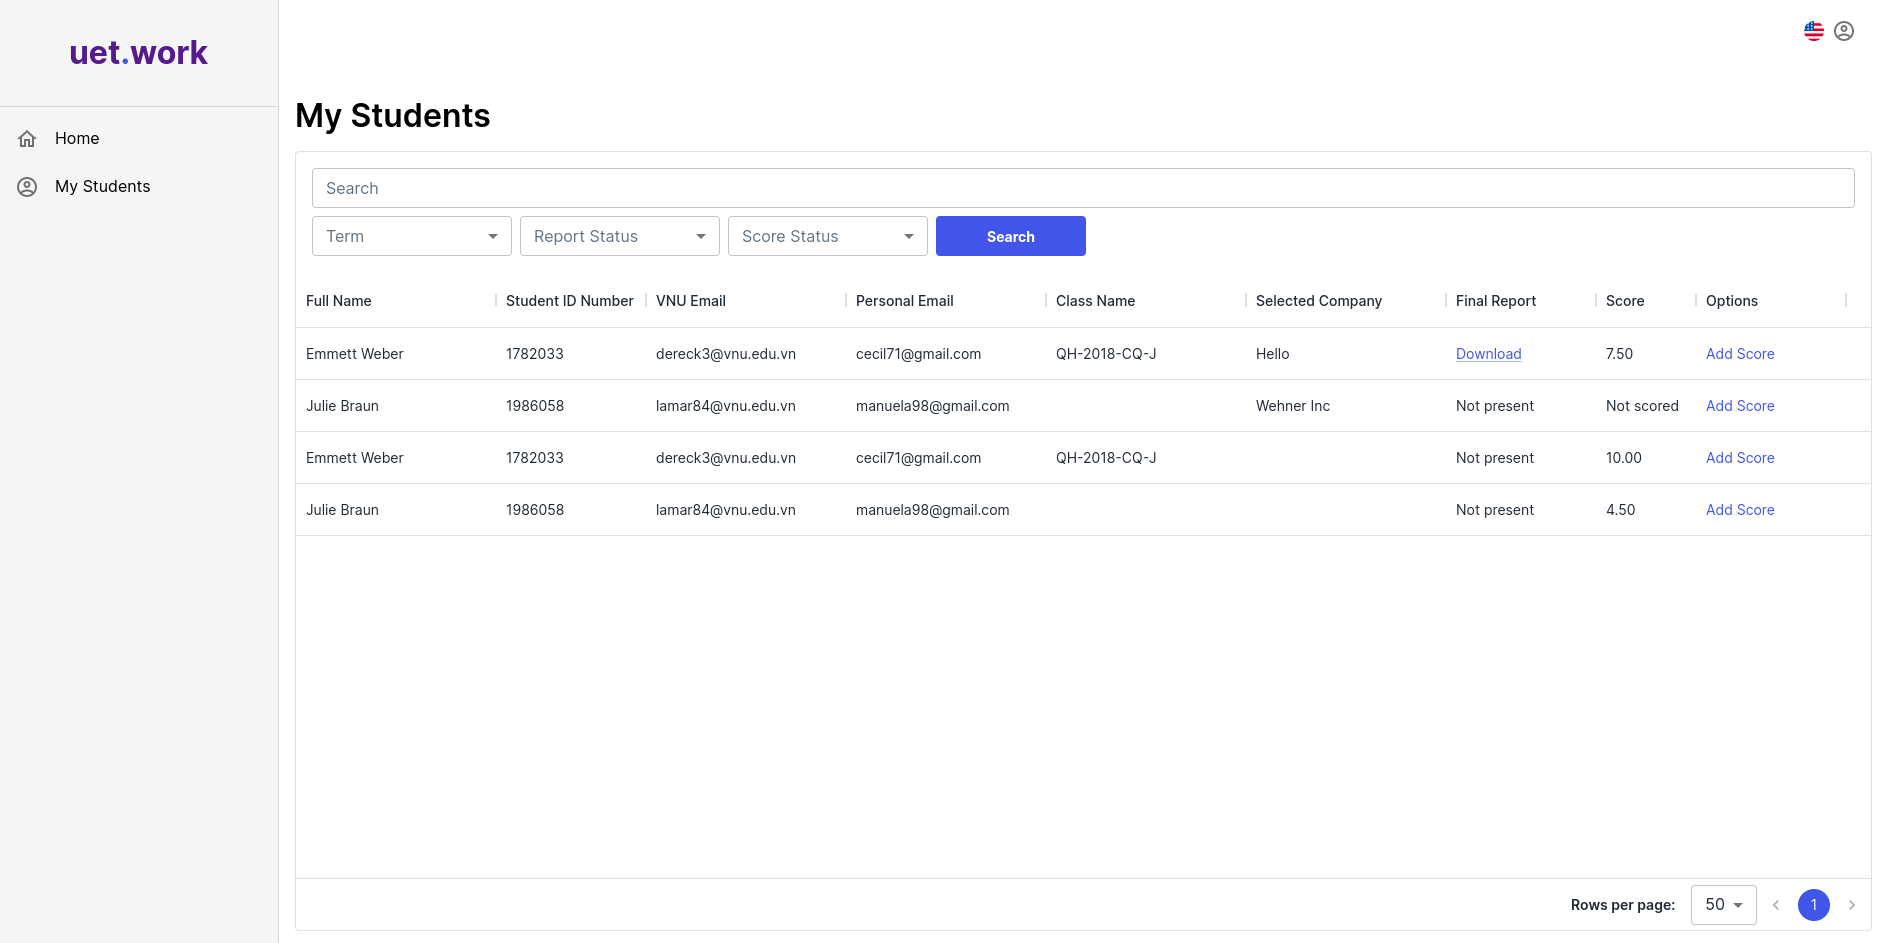
\includegraphics[width=\linewidth]{./images/image13.png}
	\caption{Màn hình hệ thống (tiếng Anh)}
	\label{fig:en_page}
\end{figure}

\begin{figure}[]
	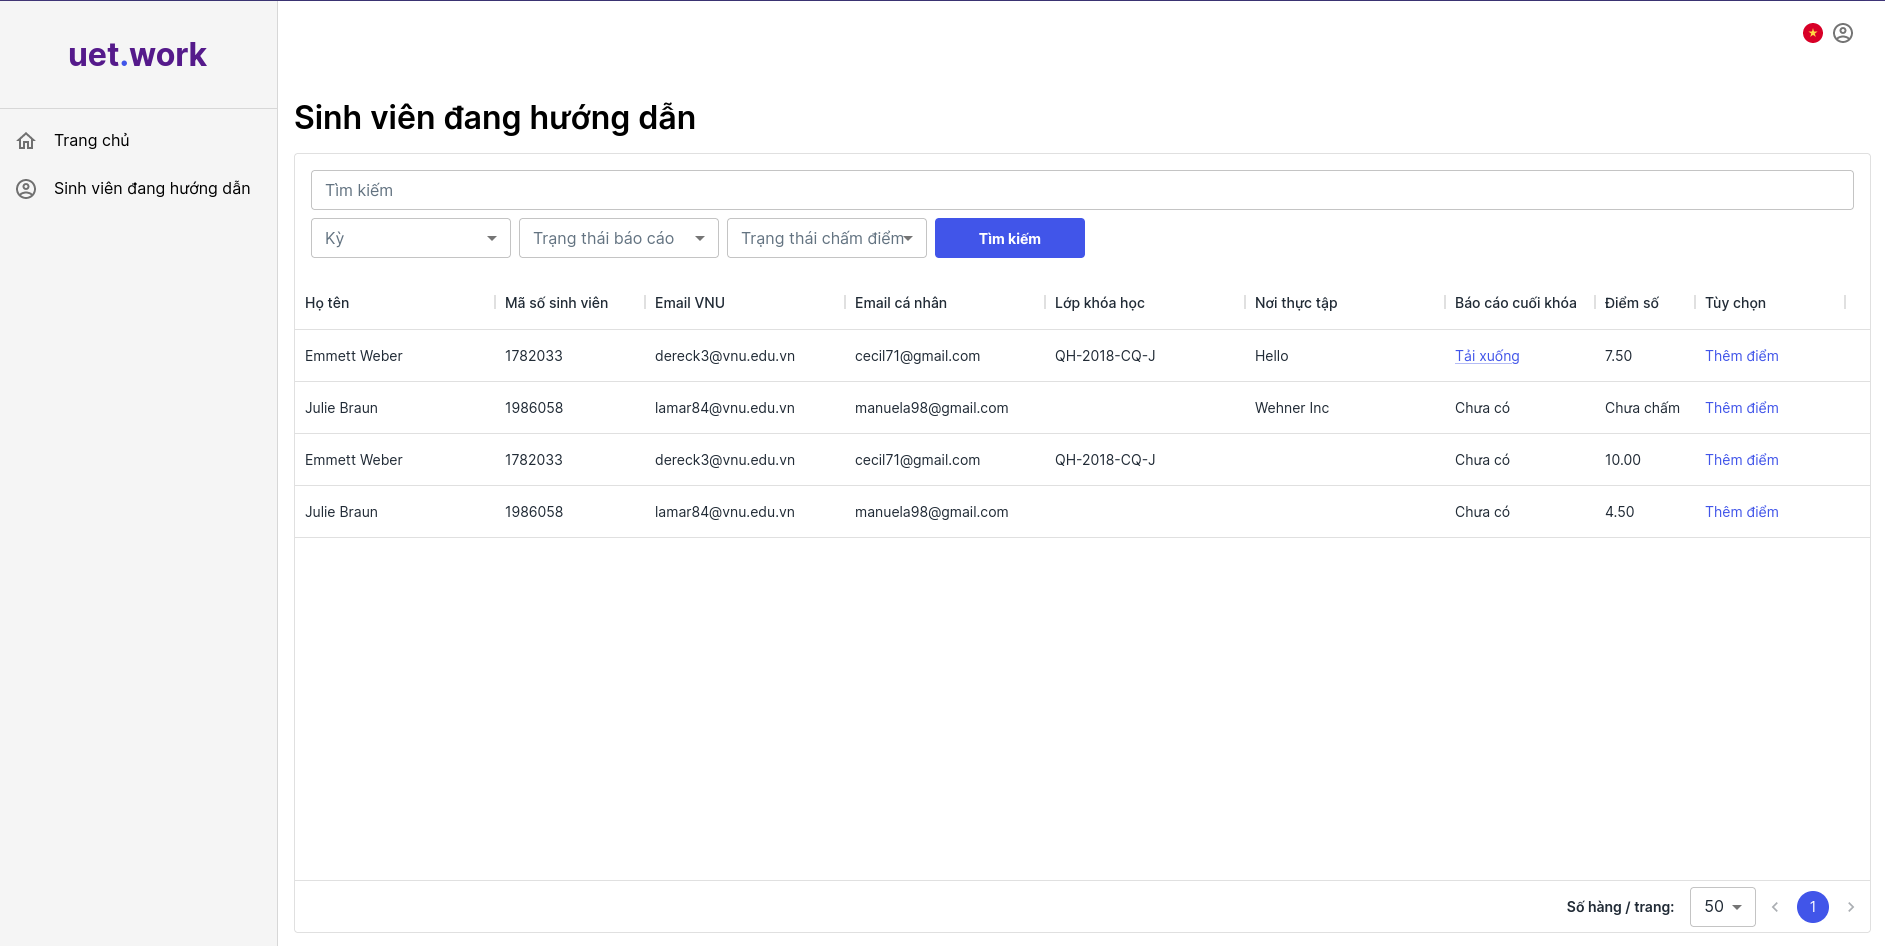
\includegraphics[width=\linewidth]{./images/image12.png}
	\caption{Màn hình hệ thống (tiếng Việt)}
	\label{fig:vi_page}
\end{figure}

\hypertarget{hux1ed7-trux1ee3-nhiux1ec1u-phux1b0ux1a1ng-thux1ee9c-ux111ux103ng-nhux1eadp}{%
\subsection{Hỗ trợ nhiều phương thức đăng
nhập}\label{hux1ed7-trux1ee3-nhiux1ec1u-phux1b0ux1a1ng-thux1ee9c-ux111ux103ng-nhux1eadp}}

Hệ thống cung cấp cho người dùng khả năng đăng nhập bằng LDAP và đăng
nhập bằng Google. Bằng cách này, nhà trường có thể tận dụng cơ sở dữ
liệu người dùng có sẵn để cho phép người dùng đăng nhập nhanh và tiện
lợi hơn.

\end{document}